% ============================================================
% PHẦN Faster-GS — Slide bổ sung 1/N: Tổng quan 5 cơ chế mới
% ============================================================

% --- Slide (mới) ---
\begin{frame}{Faster-GS (Hahlbohm et al., CVPR 2026): 5 cơ chế mới tích hợp}
\footnotesize
\begin{itemize}
    \item Repo vừa gộp thêm các cơ chế từ \textbf{Faster-GS} (Hahlbohm, Franke, Eisemann, Magnor — CVPR 2026) bên cạnh FastGS gốc, theo đúng tinh thần "luôn bật, không tuỳ chọn" (không còn cờ \texttt{if/else}).
\end{itemize}
\begin{table}
\centering
\begin{tabular}{ll}
\toprule
\textbf{Luôn bật (không cờ)} & \textbf{Giữ tắt (có chủ đích)} \\
\midrule
Fused Adam optimizer (kernel CUDA) & \\
3D anti-aliasing filter (Mip-Splatting) & MCMC densification \\
Morton Z-order reordering & \small (xung đột thuật toán với \\
Random-init fallback (thiếu COLMAP points3D) & \texttt{densify\_and\_prune\_fastgs}) \\
\bottomrule
\end{tabular}
\end{table}
\begin{itemize}
    \item MCMC densification là cơ chế thay thế đã cài đặt đầy đủ, đúng toán, nhưng \textbf{không được gọi} trong control-flow mặc định vì hai cơ chế densify không thể chạy đồng thời trên cùng tập Gaussian.
\end{itemize}
\centering
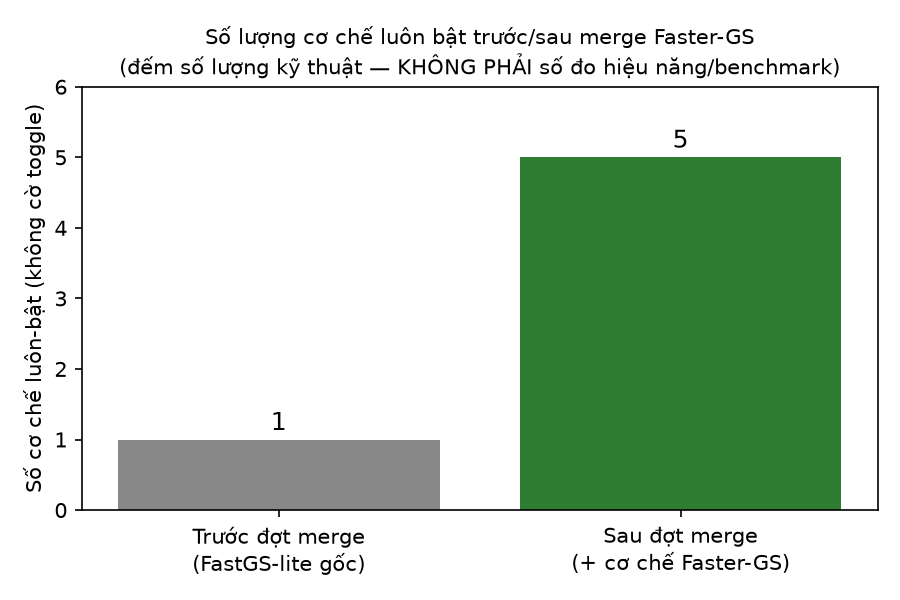
\includegraphics[width=0.3\linewidth]{../BOOK/fastergs_merge_figures/00_techniques_overview.png}
\captionof{figure}{\footnotesize Số cơ chế luôn bật trước/sau đợt merge (đếm số lượng, không phải benchmark)}
\end{frame}
